% common part for every lection

\documentclass{beamer}

\usetheme{Warsaw}
\usefonttheme[onlylarge]{structurebold}
\setbeamerfont*{frametitle}{size=\normalsize,series=\bfseries}
\setbeamertemplate{navigation symbols}{}

\usepackage{pdfpages}
\usepackage{soul}
\usepackage{ucs}
\usepackage[utf8x]{inputenc}
\usepackage[TS1,T2A]{fontenc}
\usepackage[english,russian]{babel}
\usepackage{times}
\usepackage{listings}

\author[Author, Vlad Shakhov]{Влад 'mend0za' Шахов\\Linux \& Embedded Team Leader}

\institute[SaM Solutions]
{
  Linux \& Embedded Department
}

\date[Dec 2012]

\subject{Linux QA training}

\pgfdeclareimage[height=1.5cm]{sam-solutions-logo}{clipart/sam-solutions-elinux}

\logo{\pgfuseimage{sam-solutions-logo}}

\graphicspath{{./clipart/}}


\title[SaM Solutions. Linux QA Training]
{
  Часть 1.\\
  Введение в Linux.
}

\begin{document}

\begin{frame}
  \titlepage
\end{frame}

\section{История и архитектура}

% краткая историческая справка
\begin{frame}
  \frametitle{История Linux}

  \begin{enumerate}
    \item Начало. AT\&T Unix Edition 1. 1971
    \item AT\&T Unix Edition 5. 1975. Полностью переписана на Си. 
    \item Появление BSD Unix (1978)
    \item BSD 4.2. Первая реализация TCP/IP. 1983
    \item Проект GNU. 1983 
    \item Расцвет коммерческих Unix-подобных систем. 80-е, начало 90х.
    \item AT\&T Unix System V Release 4. 1988
    \item Ядро Linux 0.01 1991 
  \end{enumerate}

\end{frame}

% архитектура классических Unix
% картинки : круговая, и прямоугольная
\begin{frame}
  \frametitle{Архитектура классических Unix}
    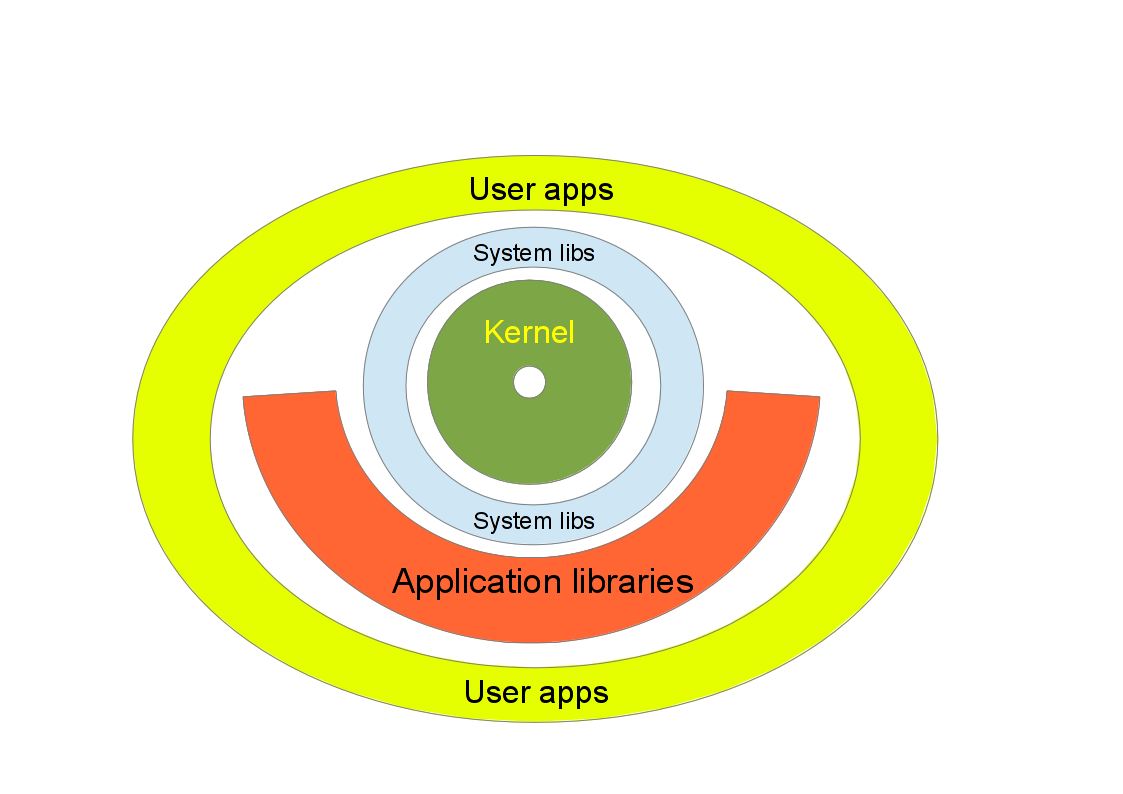
\includegraphics[height=8cm]{classic-unix-arch}
\end{frame}


\begin{frame}
  \frametitle{Архитектура Linux - 2}

  \begin{center}
    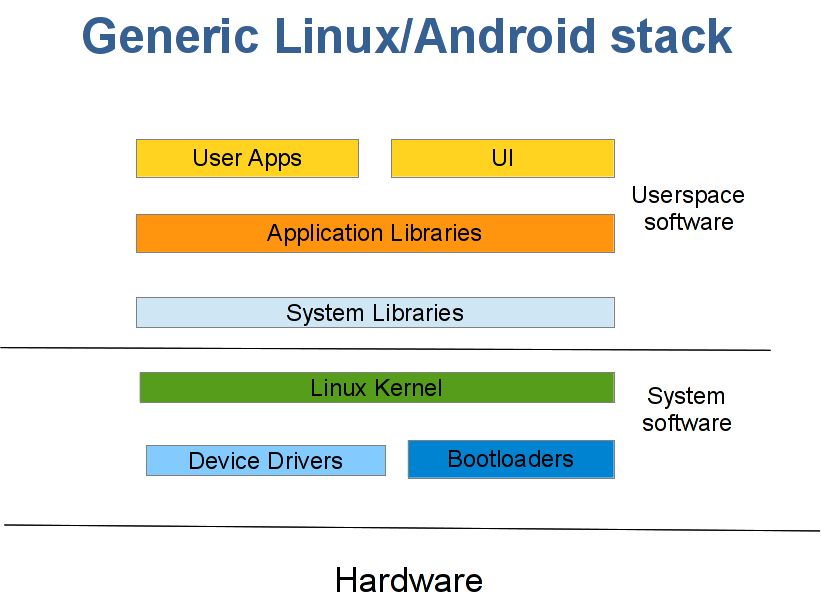
\includegraphics[height=7cm]{linux-software-stack}
  \end{center}

\end{frame}

\begin{frame}
  \frametitle{Что такое ``Linux''?}
  \begin{center}
    \alert{Что же такое ``Linux''?}
  \end{center}

  \pause 

  \emph{Linux : ядро ОС\footnote{ОС - операционная система}(узкое значение)}
  \newline
  \pause

  \emph{Linux : семейство ОС на одноимённом ядре (широкое значение)}

\end{frame}

% основные черты
\begin{frame}
  \frametitle{Основные черты Unix-подобных ОС}

  \begin{itemize}
    \item Многозадачная многопользовательская ОС.
    \item Переносимость: Код на языке Си
    \item Стандарты :
      \begin{itemize} 
	\item одинаковая структура ОС
	\item ряд стандартных, переносимых интерфейсов.
      \end{itemize}
    \item Командная строка - единый интерфейс управления.
    \item Eдиная древовидная файловая система\footnote{Через интерфейс файловой системы осуществляется доступ к данным, терминалам, принтерам, дискам, сети и даже к оперативной памяти}.
    \item Большое количество программного обеспечения.
  \end{itemize}
\end{frame}

\section{Сессия пользователя}

% пользовательская сессия
\begin{frame}
  \frametitle{Пользовательская сессия}

  \begin{center}
    \begin{block}<1->{Многопользовательская система?}
      Надо представиться системе. Логин и пароль.
    \end{block}

    \begin{block}<2->{Как может выглядеть}
      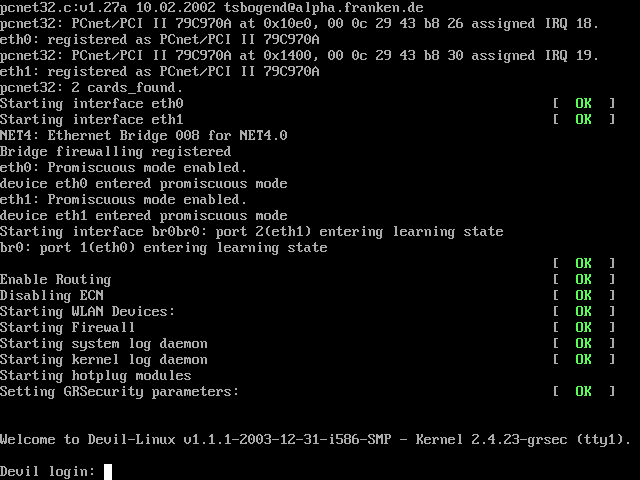
\includegraphics[height=2.5cm]{console-login-screenshot}
      
\includegraphics[height=2.5cm]{gdm-login-screenshot}
      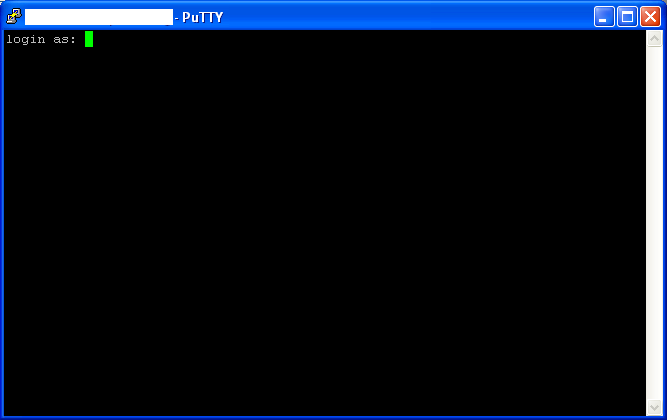
\includegraphics[height=2.5cm]{putty-login-screenshot}
    \end{block}

    \begin{block}<3->{Виды сессий}
      \begin{itemize} 
	\item локальные и удалённые (сетевые)
	\item текстовые и графические
      \end{itemize}
    \end{block}

  \end{center}

\end{frame}

\subsection{SSH}

\begin{frame}
  \frametitle{Входим удалённо. SSH}

  \begin{center}

    SSH - \emph{S}ecure \emph{SH}ell
    \newline \pause

    Протокол удалённой работы по сети для Linux.

    Много реализаций клиентов и серверов. 
    \newline
    \pause

    \emph{Как может выглядеть:} 
    \newline
    \fbox{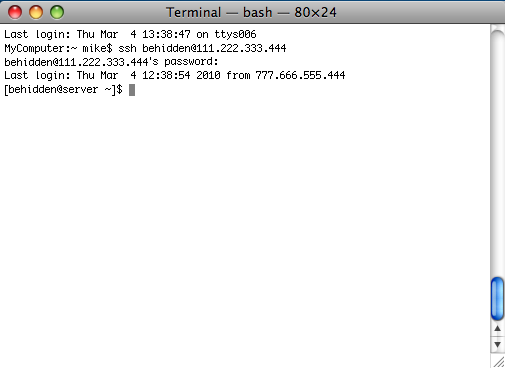
\includegraphics[height=3.5cm]{console-ssh-screenshot}}
    \emph{ }
    \fbox{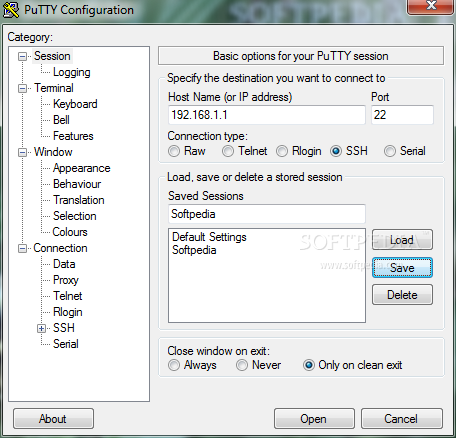
\includegraphics[height=3.5cm]{putty-config-screenshot}}
  \end{center} 

\end{frame}

\begin{frame}
  \frametitle{Выход из матрицы}
  
  \begin{center}
    
\includegraphics[height=5.5cm]{matrix-screenshot}
    \pause
    \newline
    \begin{itemize}
      \item Команда \emph{exit}
      \item Hotkey \emph{Ctrl+d}
      \item Закрыть клиента
    \end{itemize}
  \end{center}

\end{frame}

\subsection{Ключи SSH}

\begin{frame}
  \frametitle{Методы авторизации SSH. Ключи}

  \alert{Не хочешь вводить пароли?}
  \pause

  \alert{Не вводи!} 
  \pause

  \begin{center}
    Aвторизация в SSH.
    
    Пара: открытый + секретный ключ. 
    
    Вместо пароля.
  \end{center}

\end{frame}

\begin{frame}
  \frametitle{Ключи SSH. Создание}

  \begin{center}

    \begin{tabular}{ l r }
      \hbox{Linux: ssh-keygen} & \hbox{Windows: PuTTY keygen} \\
      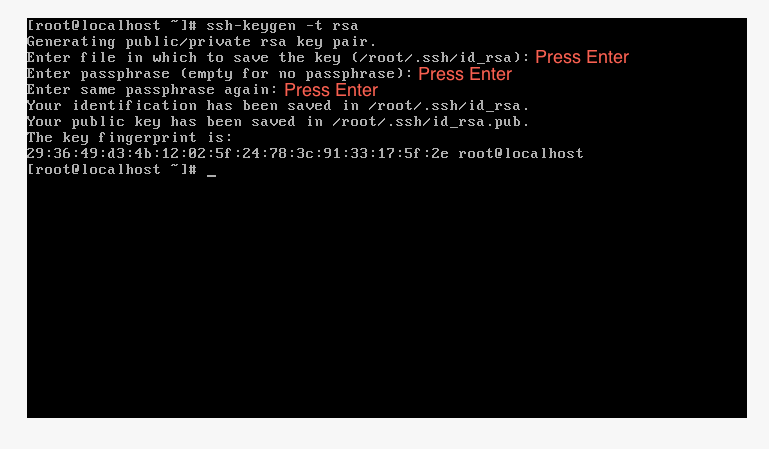
\includegraphics[height=3cm]{ssh-keygen-screenshot} & 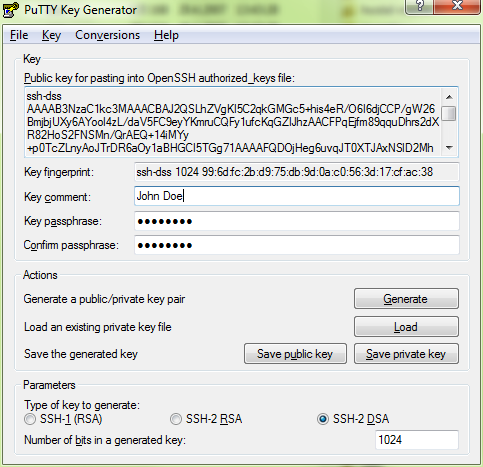
\includegraphics[height=4cm]{putty-keygen-screenshot} \\
      Ключи в папке .ssh/: & Ключи там, где сохранили \\
      id\_rsa и id\_rsa.pub &
    \end{tabular}

  \end{center}

\end{frame}

\begin{frame}
  \frametitle{Ключи SSH. Копирование}

  \begin{itemize}
    \item \alert{Что копировать?} Публичный ключ (id\_rsa.pub)  \pause
    \item \alert{Куда складывать?} в \$HOME/.ssh/authorized\_keys \newline удалённой машины \pause
    \item \alert{Как перенести?} \pause
      \begin{itemize} 
	\item Linux: ssh-copy-id username@host \pause
	\item Copy-paste в редактор \pause
      \end{itemize}
  \end{itemize}

\end{frame}

\begin{frame}
  \frametitle{SSH. Автоматизация входа}
  \begin{center}
    \begin{tabular}{ l r }
      \Large{Linux: .ssh/config} & \Large{Windows: PuTTY session} \\
      \lstinputlisting[basicstyle=\tiny]{samples/ssh-config} & \fbox{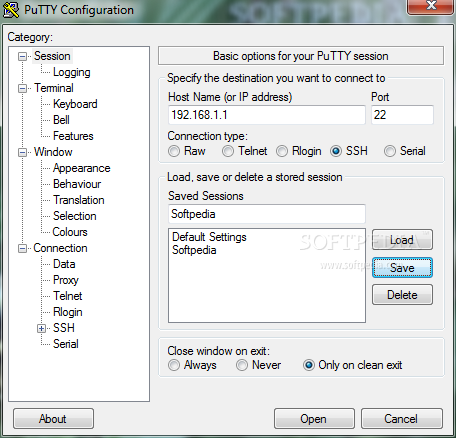
\includegraphics[height=4.5cm]{putty-config-screenshot}} \\
    \end{tabular}

  \end{center}
\end{frame}

\subsection{Unix shell}
\begin{frame}
  \frametitle{Лирическое отступление: David Korn}
  \begin{center}
    Автор Korn Shell

    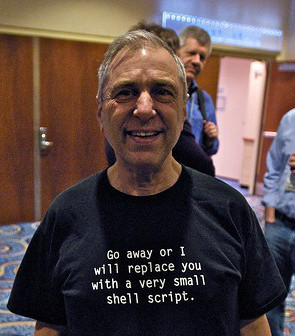
\includegraphics[height=5cm]{korn-shell-joke} 

    David Korn: ``Убирайся, или я заменю тебя очень маленьким Shell-скриптом.''
  \end{center}
\end{frame}

\begin{frame}
  \frametitle{Что такое Unix shell?}
  
  \alert{Что такое Unix shell?}

  \begin{itemize}
    \item Какие есть варианты у вас? \pause
    \item Обычная программа, запускающаяся после входа в систему \pause
    \item Интерактивный командный интерпретатор \pause
    \item Язык программирования \pause
    \item Платформа интеграции (для утилит) \pause
    \item Сотни разных реализаций (bash, ksh, zsh, tcsh, \ldots ) \pause
    \item Масса различных диалектов
  \end{itemize}

\end{frame}

\begin{frame}
  \frametitle{Life with Shell}

  \begin{center}
    \Large{готовьтесь жить вместе с Shell}
    \newline
    
    
\includegraphics[height=6cm,angle=0]{unix-power-tools-cover} 
  \end{center}

\end{frame}

\begin{frame}
  \frametitle{Получение информации о системе}
  \begin{itemize}
    \item \Large{who} и \Large{whoami} - информация о пользователях \pause
    \item \Large{free} - оперативная память \pause
    \item \Large{ps} - список процессов \pause
    \item \Large{top} - процессы в динамике \pause
    \item \Large{uptime} - время, срок работы, параметры нагрузки \pause
    \item \Large{last} - список логинившихся пользователей \pause
    \item \Large{uname -a} - информация о ядре и архитектуре
  \end{itemize}
\end{frame}

\begin{frame}[fragile]
  \frametitle{Встроенная документация}
  \begin{itemize}
    \item \Large{\alert{man}} - встроенная справка. Команды ``man'', ``apropos'', ``whatis''
      \newline Формат: \alert{page(номер раздела)}:  \verb+login(1)+\pause
    \item \alert{info - GNU texinfo}, система гипертекстовой справки \pause
    \item \alert{/usr/share/doc/*} - документация, устанавливаемая вместе с программами \pause
    \item \alert{Google} - no comments \pause
  \end{itemize}

\end{frame}

\end{document}
